%%%%%%%%%%%%%%%%%%%%%%%%%%%%%%%%%%%%%%%%%%%%%%%%%%%%%%%%%%%%%%%%%%%%%%%%%%%%%%%%
\subsection{Συμπεράσματα κεφαλαίου}

Σε αυτό το κεφάλαιο μάς απασχόλησε η ελάττωση του σφάλματος εκτίμησης στάσης
με αιτία τα ευρήματά μας στο προηγούμενο κεφάλαιο
(ενότητα \ref{subsection:02_01_05:02}). Με δεδομένο τη χρήση του φίλτρου
σωματιδίων για το έργο της παρακολούθησης της στάσης ενός ρομπότ, αναλύσαμε τη
διαθέσιμη βιβλιογραφία γύρω από την ελάττωση του σφάλματος εκτίμησης του, και
προτείναμε δύο επιπρόσθετους τρόπους με τους οποίους είναι δυνατή η επίτευξη
του στόχου. Πιο συγκεκριμένα:

\begin{itemize}
  \item Επικεντρωθήκαμε στο μοντέλο παρατηρήσεων του φίλτρου, και, σκεπτόμενοι
        αναλυτικά, θέσαμε την υπόθεση ότι η επιλογή υποσυνόλων από υποθέσεις
        στάσης του, των οποίων οι αναμενόμενες μετρήσεις από αυτές συμβαδίζουν
        περισσότερο με τις εισερχόμενες στο φίλτρο μετρήσεις του αισθητήρα
        αποστάσεων σε σχέση με άλλες υποθέσεις---η επιλογή αυτών των υποθέσεων
        στάσης ως η εκτίμηση του φίλτρου οφείλει να παράγει χαμηλότερα σφάλματα
        στάσης (ενότητα \ref{subsection:02_02_03:01}). Τα ευρήματά μας
        επιβεβαιώνουν την υπόθεση, αλλά έως ένα κατώφλι πληθικότητας αυτών των
        υποσυνόλων: στο όριο, η μοναδική υπόθεση στάσης που εμφανίζει τη
        μεγαλύτερη πιθανότητα παρατήρησης των μετρήσεων από αυτήν εμφανίζει
        μεγαλύτερα σφάλματα στάσης από ότι η συλλογική εκτίμηση του φίλτρου.
        Βάσει αυτού του ευρήματος συμπεράναμε ότι το φίλτρο σωματιδίων δεν
        αποτελεί άθροισμα υποθέσεων, αλλά μία κατακερματισμένη μορφή εκτίμησης.
  \item Ερευνήσαμε και ζητήσαμε να ελέγξουμε την ευστάθεια της υπόθεσης ότι
        το αποτέλεσμα της εφαρμογής του μετασχηματισμού της ευθυγράμμισης
        μετρήσεων δισδιάστατου αισθητήρα lidar με σαρώσεις χάρτη από την
        παραγώμενη εκτίμηση του φίλτρου στην ίδια την εκτίμηση του εμφανίζει
        χαμηλότερα σφάλματα εκτίμησης στάσης σε σχέση με την αρχική εκτίμηση
        (ενότητα \ref{subsection:02_02_03:02}). Με βάση τη διαμόρφωση της
        πειραματικής διαδικασίας, τα ευρήματα αποδεικνύουν ότι η εφαρμογή της
        διαδικασίας ευθυγράμμισης έχει σημαντικά οφέλη στην ελάττωση του
        σφάλματος εκτίμησης.
  \item Παρακινούμενοι από ελλείψεις και μεινοκτήματα μεθόδων της τρέχουσας
        βιβλιογραφίας προτείναμε έναν τρόπο ανάδρασης του αποτελέσματος της
        ευθυγράμμισης μετρήσεων με σαρώσεις χάρτη στον πληθυσμό του φίλτρου
        σωματιδίων (ενότητα \ref{subsection:02_02_03:03}): δεδομένων ότι το
        αποτέλεσμα της ευθυγράμμισης (α) είναι πιο ακριβές από την εκτίμηση του
        φίλτρου και (β) είναι άγνωστο στο ίδιο το φίλτρο, σχεδιάσαμε έναν
        μηχανισμό ανάδρασης που (i) προκαλεί πιο γρήγορη σύγκλιση και
        χαμηλότερα σφάλματα εκτίμησης σε σχέση με έναν μηχανισμό ανάδρασης της
        βιβλιογραφίας, (ii) προκαλεί την αποφυγή απόκλισης του φίλτρου σε σχέση
        με έναν δεύτερο μηχανισμό ανάδρασης της βιβλιογραφίας, και (iii)
        εμφανίζει χαμηλότερα σφάλματα στάσης σε σχέση με το φίλτρο σε κατάσταση
        ανοιχτού βρόχου.
\end{itemize}

Στο σχήμα \ref{fig:02_02_05:01} απεικονίζονται συνοπτικά οι συμβολές του
παρόντος κεφαλαίου στη μεθοδολογία ελάττωσης του σφάλματος εκτίμησης φίλτρου
σωματιδίων με χρήση αισθητήρων απόστασης τύπου 2D lidar.



\begin{figure}
  \hspace{-1cm}
  % GNUPLOT: LaTeX picture with Postscript
\begingroup
  \makeatletter
  \providecommand\color[2][]{%
    \GenericError{(gnuplot) \space\space\space\@spaces}{%
      Package color not loaded in conjunction with
      terminal option `colourtext'%
    }{See the gnuplot documentation for explanation.%
    }{Either use 'blacktext' in gnuplot or load the package
      color.sty in LaTeX.}%
    \renewcommand\color[2][]{}%
  }%
  \providecommand\includegraphics[2][]{%
    \GenericError{(gnuplot) \space\space\space\@spaces}{%
      Package graphicx or graphics not loaded%
    }{See the gnuplot documentation for explanation.%
    }{The gnuplot epslatex terminal needs graphicx.sty or graphics.sty.}%
    \renewcommand\includegraphics[2][]{}%
  }%
  \providecommand\rotatebox[2]{#2}%
  \@ifundefined{ifGPcolor}{%
    \newif\ifGPcolor
    \GPcolorfalse
  }{}%
  \@ifundefined{ifGPblacktext}{%
    \newif\ifGPblacktext
    \GPblacktexttrue
  }{}%
  % define a \g@addto@macro without @ in the name:
  \let\gplgaddtomacro\g@addto@macro
  % define empty templates for all commands taking text:
  \gdef\gplfronttext{}%
  \makeatother
  \ifGPblacktext
    % no textcolor at all
    \def\colorrgb#1{}%
    \def\colorgray#1{}%
  \else
    % gray or color?
    \ifGPcolor
      \def\colorrgb#1{\color[rgb]{#1}}%
      \def\colorgray#1{\color[gray]{#1}}%
      \expandafter\def\csname LTw\endcsname{\color{white}}%
      \expandafter\def\csname LTb\endcsname{\color{black}}%
      \expandafter\def\csname LTa\endcsname{\color{black}}%
      \expandafter\def\csname LT0\endcsname{\color[rgb]{1,0,0}}%
      \expandafter\def\csname LT1\endcsname{\color[rgb]{0,1,0}}%
      \expandafter\def\csname LT2\endcsname{\color[rgb]{0,0,1}}%
      \expandafter\def\csname LT3\endcsname{\color[rgb]{1,0,1}}%
      \expandafter\def\csname LT4\endcsname{\color[rgb]{0,1,1}}%
      \expandafter\def\csname LT5\endcsname{\color[rgb]{1,1,0}}%
      \expandafter\def\csname LT6\endcsname{\color[rgb]{0,0,0}}%
      \expandafter\def\csname LT7\endcsname{\color[rgb]{1,0.3,0}}%
      \expandafter\def\csname LT8\endcsname{\color[rgb]{0.5,0.5,0.5}}%
    \else
      % gray
      \def\colorrgb#1{\color{black}}%
      \def\colorgray#1{\color[gray]{#1}}%
      \expandafter\def\csname LTw\endcsname{\color{white}}%
      \expandafter\def\csname LTb\endcsname{\color{black}}%
      \expandafter\def\csname LTa\endcsname{\color{black}}%
      \expandafter\def\csname LT0\endcsname{\color{black}}%
      \expandafter\def\csname LT1\endcsname{\color{black}}%
      \expandafter\def\csname LT2\endcsname{\color{black}}%
      \expandafter\def\csname LT3\endcsname{\color{black}}%
      \expandafter\def\csname LT4\endcsname{\color{black}}%
      \expandafter\def\csname LT5\endcsname{\color{black}}%
      \expandafter\def\csname LT6\endcsname{\color{black}}%
      \expandafter\def\csname LT7\endcsname{\color{black}}%
      \expandafter\def\csname LT8\endcsname{\color{black}}%
    \fi
  \fi
  \setlength{\unitlength}{0.0500bp}%
  \begin{picture}(10000.00,4000.00)%
    \gplgaddtomacro\gplfronttext{%
      \colorrgb{0.00,0.00,0.00}%
      \put(1168,440){\makebox(0,0)[r]{\strut{}$0.005$}}%
      \colorrgb{0.00,0.00,0.00}%
      \put(1168,1526){\makebox(0,0)[r]{\strut{}$0.010$}}%
      \colorrgb{0.00,0.00,0.00}%
      \put(1168,2613){\makebox(0,0)[r]{\strut{}$0.015$}}%
      \colorrgb{0.00,0.00,0.00}%
      \put(1300,220){\makebox(0,0){\strut{}$200$}}%
      \colorrgb{0.00,0.00,0.00}%
      \put(2091,220){\makebox(0,0){\strut{}$600$}}%
      \colorrgb{0.00,0.00,0.00}%
      \put(2882,220){\makebox(0,0){\strut{}$1000$}}%
      \colorrgb{0.00,0.00,0.00}%
      \put(5000,4600){\makebox(0,0){\strut{}Μέσο σφάλμα εκτίμησης σε $N = 100$ διαδρομές ανά εκτιμώμενη στάση}}%
      \colorrgb{0.00,0.00,0.00}%
      \put(5100,-510){\makebox(0,0){\strut{}Αριθμός εκτιμήσεων στάσης στο χρόνο}}%
      \definecolor{gr}{RGB}{161,214,107}
      \definecolor{pi}{RGB}{232,163,201}
      \definecolor{k}{RGB}{0,0,0}
      \definecolor{sm}{RGB}{227,74,51}
      \put(2110,4229){\makebox(0,0){\strut{}{\color{k}{\rule[0.6mm]{0.5cm}{0.5mm}}} MCL}}
      \put(2200,4000){\makebox(0,0){\strut{}{\color{gr}{\rule[0.6mm]{0.5cm}{0.5mm}}} $\%$MCL}}
      \put(1900,4000){\makebox(0,0){\strut{}{\color{pi}{\rule[0.6mm]{0.25cm}{0.5mm}}}}}

      \put(4700,4229){\makebox(0,0){\strut{}{\color{k}{\rule[0.6mm]{0.5cm}{0.5mm}}} MCL}}
      \put(5100,4000){\makebox(0,0){\strut{}{\color{sm}{\rule[0.6mm]{0.5cm}{0.5mm}}} MCL $\circ$ smsm}}

      \put(7460,4229){\makebox(0,0){\strut{}{\color{k}{\hdashrule[0.6mm]{0.60cm}{0.5mm}{0.5mm}}} MCL}}
      \put(8100,4000){\makebox(0,0){\strut{}{\color{k}{\rule[0.6mm]{0.5cm}{0.5mm}}} MCL $\circ$ smsm $\circ$ $\circlearrowleft$}}

      \put(2210,-100){\makebox(0,0){\strut{} CORRIDOR}}
      \put(5000,-100){\makebox(0,0){\strut{} WAREHOUSE}}
      \put(7990,-100){\makebox(0,0){\strut{} WAREHOUSE}}
    }%
    \gplgaddtomacro\gplfronttext{%
    }%
    \gplgaddtomacro\gplfronttext{%
      \colorrgb{0.00,0.00,0.00}%
      \put(4053,440){\makebox(0,0)[r]{\strut{}$0$}}%
      \colorrgb{0.00,0.00,0.00}%
      \put(4053,1092){\makebox(0,0)[r]{\strut{}$0.02$}}%
      \colorrgb{0.00,0.00,0.00}%
      \put(4053,1744){\makebox(0,0)[r]{\strut{}$0.04$}}%
      \colorrgb{0.00,0.00,0.00}%
      \put(4053,2395){\makebox(0,0)[r]{\strut{}$0.06$}}%
      \colorrgb{0.00,0.00,0.00}%
      \put(4053,3047){\makebox(0,0)[r]{\strut{}$0.08$}}%
      \colorrgb{0.00,0.00,0.00}%
      \put(4053,3699){\makebox(0,0)[r]{\strut{}$0.10$}}%
      \colorrgb{0.00,0.00,0.00}%
      \put(4185,220){\makebox(0,0){\strut{}$0$}}%
      \colorrgb{0.00,0.00,0.00}%
      \put(4734,220){\makebox(0,0){\strut{}$100$}}%
      \colorrgb{0.00,0.00,0.00}%
      \put(5284,220){\makebox(0,0){\strut{}$200$}}%
      \colorrgb{0.00,0.00,0.00}%
      \put(5833,220){\makebox(0,0){\strut{}$300$}}%
    }%
    \gplgaddtomacro\gplfronttext{%
      \colorrgb{0.00,0.00,0.00}%
      \put(6939,440){\makebox(0,0)[r]{\strut{}$0$}}%
      \colorrgb{0.00,0.00,0.00}%
      \put(6939,1092){\makebox(0,0)[r]{\strut{}$0.02$}}%
      \colorrgb{0.00,0.00,0.00}%
      \put(6939,1744){\makebox(0,0)[r]{\strut{}$0.04$}}%
      \colorrgb{0.00,0.00,0.00}%
      \put(6939,2395){\makebox(0,0)[r]{\strut{}$0.06$}}%
      \colorrgb{0.00,0.00,0.00}%
      \put(6939,3047){\makebox(0,0)[r]{\strut{}$0.08$}}%
      \colorrgb{0.00,0.00,0.00}%
      \put(6939,3699){\makebox(0,0)[r]{\strut{}$0.10$}}%
      \colorrgb{0.00,0.00,0.00}%
      \put(7071,220){\makebox(0,0){\strut{}$0$}}%
      \colorrgb{0.00,0.00,0.00}%
      \put(7620,220){\makebox(0,0){\strut{}$100$}}%
      \colorrgb{0.00,0.00,0.00}%
      \put(8170,220){\makebox(0,0){\strut{}$200$}}%
      \colorrgb{0.00,0.00,0.00}%
      \put(8719,220){\makebox(0,0){\strut{}$300$}}%
    }%
    \put(0,0){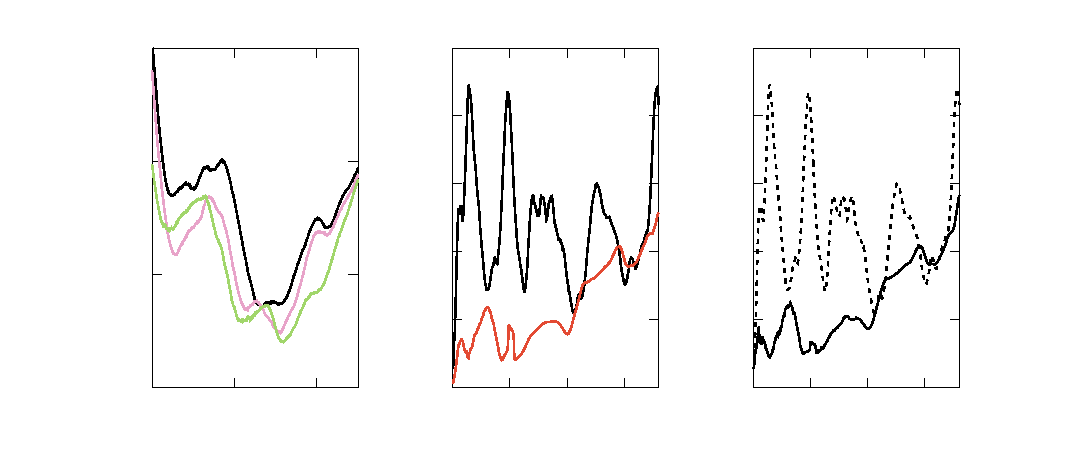
\includegraphics{./figures/parts/02/chapters/02/sections/05/h_123}}%
    \gplfronttext
  \end{picture}%
\endgroup

  \vspace{1cm}
  \caption{\small Η συμβολή των μεθόδων που παρουσιάστηκαν στο παρόν κεφάλαιο
           ως προς το μέσο σφάλμα εκτίμησης ανά στάση στα διενεργηθέντα
           πειράματα. Αριστερά: με μαύρο χρώμα το αποτέλεσμα του MCL και με άλλα
           χρώματα το αποτέλεσμα της επιλογής υποσυνόλων σωματιδίων στο
           περιβάλλον CORRIDOR. Μέση: με μαύρο χρώμα το αποτέλεσμα του MCL και
           με κόκκινο το αποτέλεσμα της ευθυγράμμισης μετρήσεων δισδιάστατου
           αισθητήρα lidar με σαρώσεις χάρτη (smsm). Δεξιά: με διακεκομμένη
           γραμμή το αποτέλεσμα του MCL και με συνεχή το αποτέλεσμα του ολικού
           συστήματος (σχήμα \ref{fig:overall_system}) μετά την ανατροφοδότηση
           του αποτελέσματος της ευθυγράμμισης μετρήσεων με σαρώσεις χάρτη
           στον πληθυσμό του φίλτρου μέσω της προτεινόμενης μεθόδου
           ανατροφοδότησης}
  \label{fig:02_02_05:01}
\end{figure}


%%%%%%%%%%%%%%%%%%%%%%%%%%%%%%%%%%%%%%%%%%%%%%%%%%%%%%%%%%%%%%%%%%%%%%%%%%%%%%%%
\subsection{Αιτίες περαιτέρω έρευνας}


smsm οχι μονη της χωρις φιλτρο σωματιδιων (hard loop closure τα γαμαει τη μανα)
